\documentclass[letterpaper,10pt]{article}
\usepackage{graphicx}
\usepackage{osameet2}
\usepackage{amsmath,amssymb}


\begin{document}
\title{Objective-first design of 
    high-efficiency, small-footprint couplers between 
    arbitrary nanophotonic waveguide modes}
\author{Jesse Lu$^\ast$ and Jelena Vu\v{c}kovi\'{c}}
\address{Stanford University, Stanford, California, USA.}
\email{\url{jesselu@stanford.edu}}

\maketitle
\begin{abstract}
We present an algorithm for designing
    high efficiency ($\sim$98\%), 
    small-footprint (1.5-4 square vacuum wavelengths)
    couplers between arbitrary nanophotonic waveguide modes
    in two dimensions.
Our ``objective-first'' method is
    computationally fast (15 minutes on a single-core personal computer), 
    requires no trial-and-error, and
    does not require guessing a good starting design.
We demonstrate designs for various coupling problems which suggest 
    that our method allows for the design of any 
    single-mode, linear optical device.
\end{abstract}
\ocis{230.75370, 130.3990.}

\begin{thebibliography}{99}
\bibitem{fibergrating} Y. Tang, Z. Wang, L. Wosinski, U. Westergren, and S. He,
    ``Highly efficient nonuniform grating coupler for silicon-on-insulator 
    nanophotonic circuits,''
    Opt. Lett. \textbf{35}, 1290-1292 (2010).
\bibitem{ridge}  K. K. Lee, D. R. Lim, L.C. Kimerling, J. Shin, and F. Cerrina, 
    ``Fabrication of ultralow-loss Si/SiO2 waveguides by roughness reduction,''
    Opt. Lett. \textbf{26}, 1888-1890 (2001).
\bibitem{pcslow} Y. A. Vlasov, M. O'Boyle, H. F. Hamann, and S. J. McNab,
    ``Active control of slow light on a chip with photonic crystal waveguides,''
    Nature \textbf{438}, 65-69 (2005).
\bibitem{slotfocus} M. Lipson, 
    ``Guiding, modulating, and emitting light on 
    silicon-challenges and opportunities,'' 
    J. Lightwave Technol. \textbf{23}, 4222-4238 (2005).
\bibitem{active} J. Van Campenhout, P. Rojo Romeo, P. Regreny, C. Seassal, 
    D. Van Thourhout, S. Verstuyft, L. Di Cioccio, J.-M. Fedeli, 
    C. Lagahe, and R. Baets, 
    ``Electrically pumped InP-based microdisk lasers integrated with a 
    nanophotonic silicon-on-insulator waveguide circuit,'' 
    Opt. Express \textbf{15}, 6744-6749 (2007).
\bibitem{metallic} L. Tang, S. E. Kocabas, S. Latif, A. K. Okyay, 
    D. S. Ly-Gagnon, K. C. Saraswat, and D. A. B. Miller, 
    ``Nanometre-scale germanium photodetector enhanced by a 
    near-infrared dipole antenna,'' 
    Nature Photonics \textbf{2}, 226 – 229 (2008).
% \bibitem{fwadia} V. R. Almeida, R. R. Panepucci, and M. Lipson, 
%     ``Nanotaper for compact mode conversion,'' 
%     Opt. Lett. \textbf{28}, 1302-1304 (2003) 
% \bibitem{wwadia} S. G. Johnson, P. Bienstman,  M. A. Skorobogatiy, 
%     M. Ibanescu1, E. Lidorikis, and J. D. Joannopoulos,
%     ``Adiabatic theorem and continuous coupled-mode theory for 
%     efficient taper transitions in photonic crystals,''
%     Phys. Rev. E \textbf{66}, 066608 (2002)
% \bibitem{deriv} F. Wang, J. S. Jensen, O. Sigmund, 
%     ``Robust topology optimization of photonic crystal waveguides with 
%     tailored dispersion properties.'' 
%     J. Opt. Soc. Am. B \textbf{28}, 387-397 (2011)
% \bibitem{boydbook} S. Boyd, and L. Vandenberghe, 
%     \emph{Convex Optimization} 
%     (Cambridge University Press, 2004)
\bibitem{prevwork} J. Lu, S. Boyd, and J. Vuckovic, 
    ``Inverse design of a three-dimensional nanophotonic resonator,''
    Opt. Express \textbf{19}, 10563-10.750 (2011). 
\bibitem{code} \url{www.github.com/JesseLu/objective-first}
\end{thebibliography}

\section{Motivation}

% Why is waveguide mode conversion important?
Optical mode conversion, 
    the efficient transfer of photons from one guided mode to another,
    is a fundamental requirement in nanophotonics.
For instance, efficient conversion between waveguides modes
    is essential for:
    \begin{itemize}
        \item Coupling to and from optical fiber\cite{fibergrating}, 
        to communicate with the outside world.
    \item Coupling between various nanophotonic waveguides, 
        since different waveguides are best suited for different applications.
        For example, ridge waveguides seem ideal for 
            low-loss transport\cite{ridge},
            but other waveguides, 
            such as photonic crystal waveguides or slot waveguides,
            may be better suited for slow-light\cite{pcslow} 
            or nonlinear optical devices based on 
            localized field intensities\cite{slotfocus}.
    \item Coupling between different materials systems such as
       passive, active\cite{active}, and metallic\cite{metallic} devices. 
    \end{itemize}
In fact, the problem of converting between nanophotonic modes is essentially
    the function of all linear nanophotonic devices, since
    any linear device is completely characterized by its input and output modes
    and the coupling coefficients between them.

In this paper, we present a method to solve the problem 
    of designing single-mode, linear nanophotonic devices.
We then demonstrate this method by designing coupling structures 
    between various nanophotonic waveguides.
Furthermore, we show that our method 
     does not require a good initial design,
     is computationally fast,
     and can generate high efficiency couplers within a very small footprint. 
% 
% 
% % Why are current solutions insufficient?
% % Brute force
% Of the design strategies currently available,
%     brute-force parameter search is the most often employed 
%     because of its sheer simplicity.
% Although it may be suitable for tuning existing designs,
%     the parameter space for most practical devices is simply too large
%     for such a strategy to be tractable.
% 
% % Adiabatic mode conversion (large devices, symmetry breaking)
% Adiabatic mode conversion strategies have been succesful
%     for certain fiber-waveguide\cite{fwadia} and 
%     waveguide-waveguide\cite{wwadia} couplers,
%     even if the resulting devices often require large footprints.
% However, adiabatic approaches cannot be used in many important cases 
%     such as coupling in the out-of-plane direction, or
%     coupling between modes of opposite symmetry.

% How does your algorithm solve this problem?
% \subsection{Advantages of objective-first design}
\section{Objective-first approach}
% What is objective-first optimization?
Physical structures are typically designed by solving the following problem:
    \begin{subequations}\label{eq:adj}
    \begin{align} 
    \text{decrease} & \quad f(x) \label{eq:adj:obj} \\ 
    \text{subject to} & \quad g(x,p) = 0, \label{eq:adj:con}
    \end{align}
    \end{subequations}
    where $x$ is the field variable and $p$ is the structure variable.
Here, $f(x)$, the \emph{design objective}, 
    calculates the performance of the device 
    (e.g. amount of power lost); 
    while $g(x,p)$ is the underlying physical equation for the system
    (e.g. the electromagnetic wave equation).

In contrast, the objective-first approach solves 
    \begin{subequations}\label{eq:ob1}
    \begin{align} 
    \text{decrease} & \quad \|g(x,p)\|^2 \label{eq:ob1:obj} \\ 
    \text{subject to} & \quad f(x) = 0, \label{eq:ob1:con}
    \end{align}
    \end{subequations}
    where $\|g(x,p)\|^2$ is the \emph{physics residual}.
We term this formulation ``objective-first''
    because the design objective is prioritized even above satisfying physics;
    specifically, we force our design to always exhibit the desired performance
    ($f(x) = 0$), even at the expense of
    not perfectly satisfying the underlying physics which governs its operation.

The motivation behind this formulation is two-fold.
First, this approach allows one to arrive at a locally-optimal design rapidly 
    by allowing $x$ and $p$ to vary independently, 
    as opposed to Eq.~\ref{eq:adj}
    where the value of $x$ is completely dependent on $p$.
Second, it enables an increase in the likelihood of 
    arriving at a high efficiency design
    by forcibly imposing $f(x) = 0$,
    and thereby circumvents any local optima consisting of
    low-performance devices.

% How is it applied to waveguide coupler design?
\section{Objective-first design of waveguide couplers}
We now demonstrate the objective-first approach
    by designing waveguide couplers in two-dimensions.
Specifically, we work in the two-dimensional transverse electric mode,
    choosing $H_z$ as the field variable $x$,
    and $\epsilon^{-1}$ (the inverse of the permittivity) 
    as the structure variable $p$.
This results in the following form of the physics residual,
    \begin{equation}
    \|g(x,p)\|^2 = 
    \|g(H_z, \epsilon^{-1})\|^2 = 
    \| \nabla \times \epsilon^{-1} \nabla \times H_z - \mu_0 \omega^2 H_z \|^2,
    \end{equation}
    where $\omega$ is the angular frequency,
    and $\mu_0$ is the permeability of free-space.

In order to produce a method applicable 
    to the design of any linear nanophotonic device,
    we note that its performance
    will be completely characterized by the fields along its boundary,
    and therefore, 
    we choose a boundary-value formulation for the design objective 
    as shown in Fig.~\ref{fig:intro}.
Namely, we first compute the boundary fields needed to obtain
    perfect performance, $H_z^\text{perfect}$,
    and then form the design objective as
    \begin{equation}
    f(x) = f(H_z) = \begin{bmatrix}
        H_z - H_z^\text{perfect} \\
        \frac{\partial H_z}{\partial n} - 
            \frac{\partial H_z^\text{perfect}}{\partial n}
        \end{bmatrix}_\text{boundary}
        = 0,
    \end{equation}
    where $\partial H_z / \partial n$ 
    denotes the spatial derivative in the direction normal to the boundary.

\begin{figure}[htb]
    \centering
    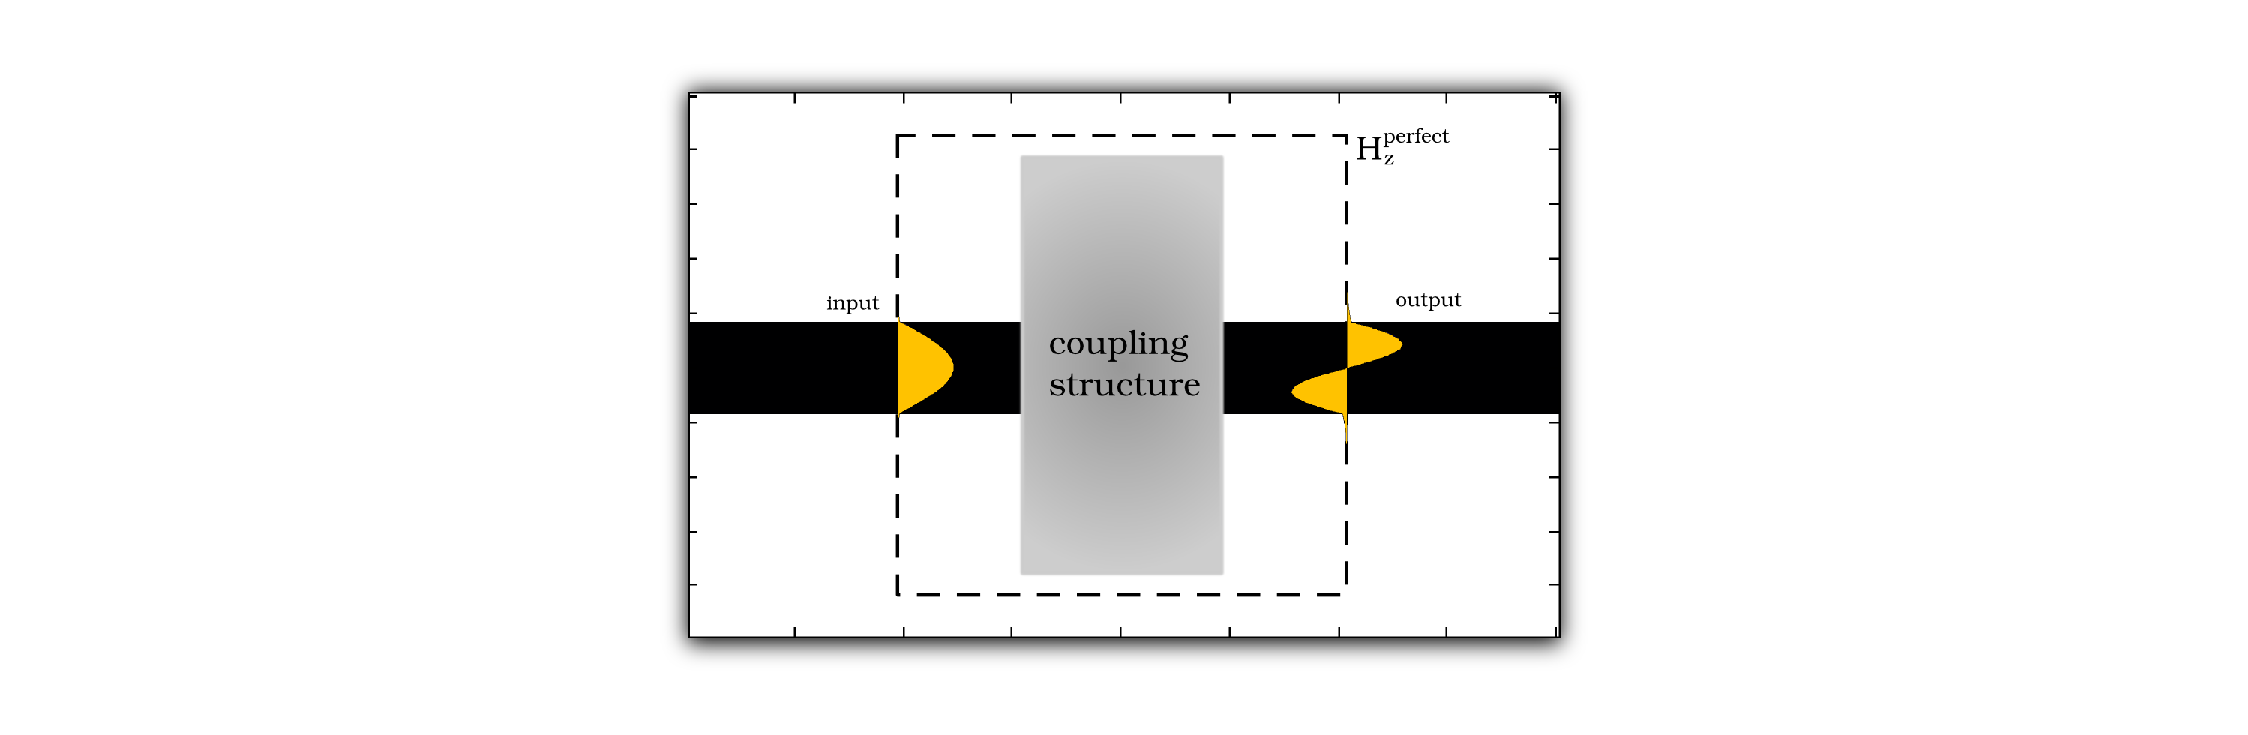
\includegraphics[width=\textwidth]{intro} 
    \caption{Boundary-value formulation of the design objective.
        The values of $H_z^\text{perfect}$, 
            defined along the dashed box surrounding the design area
            (coupling structure), 
            are shown in orange. 
        The values of $H_z^\text{perfect}$ along the top and bottom edges
            of the dashed box are set to zero.
        In this schematic, the fundamental and second-order waveguide modes
            have been chosen as the input and output modes respectively.}
    \label{fig:intro}
\end{figure}
    
Such a design objective is both extremely simple and widely adaptable 
    to the design of linear nanophotonic devices in general.
Additionally, it is trivial to enforce,
    often requiring only that we overwrite boundary field values.
On the other hand, such a formulation often prohibits the physics residual 
    from disappearing completely; 
    however, we find that very good device performance is still obtained
    as long as the physics residual is sufficiently small.

Lastly, we employ an alternating directions strategy,
    where both $x$ and $p$ are solved iteratively\cite{prevwork}
    and limit the allowable values of $\epsilon$ to be between
    the permittivity of vacuum and of silicon,
    \begin{equation}
    \epsilon_0 \le \epsilon \le \epsilon_\text{silicon}.
    \end{equation}
Note that a completely binary structure,
    where $\epsilon = \{\epsilon_0, \epsilon_\text{silicon}\}$,
    is needed for manufacturing purposes; this will be pursued in a future work.
That said, the final designs presented here 
    all have significant portions which are already binary.


\subsection{Coupler designs}
We now present five results which suggest our method
    is indeed able to design arbitrary single-mode, linear nanophotonic devices.
These results comprise of couplers between 
    the following nanophotonic waveguides:
    \begin{enumerate}
    \item coupling between waveguides of different refractive index and width
        (Fig.~\ref{fig:fiber});
    \item coupling between waveguide modes of different order and symmetry
        (Fig.~\ref{fig:mode});
    \item coupling between waveguides that confine light 
        using different principles 
        (index guided vs. distributed Bragg reflection guided), 
        i.e., between a slab waveguide and a photonic crystal fiber
        (Fig.~\ref{fig:aircore})
    \item coupling from a dielectric to a plasmonic metal-insulator-metal 
        waveguide (Fig.~\ref{fig:mim}); and
    \item coupling from a dielectric waveguide to a (plasmonic) metal wire
        (Fig.~\ref{fig:wire}).
    \end{enumerate}
All the designs presented are both highly efficient 
    ($\sim 98\%$ coupling efficiency)
    and extremely compact 
    (with footprints of only 1.5-4 square vacuum wavelengths).
In addition, good starting points were not required; 
    all initial designs were simply $\epsilon = 9$ everywhere
    (a somewhat arbitrary guess, other values work as well).
Finally, only 15 minutes on a single-core personal computer
    were needed to obtain each design.

In the appendix, we further demonstrate the generality of our method
    by presenting several additional examples including
    \begin{enumerate}
    \item coupling between all four modes of a wide dielectric waveguide;
    \item coupling from a wide, low-index waveguide to the output waveguides in 
        Figs~\ref{fig:mode}-\ref{fig:wire}; and
    \item coupling to selected channels of a set of five plasmonic waveguides.
    \end{enumerate}

\begin{figure}[htb]
    \centering
    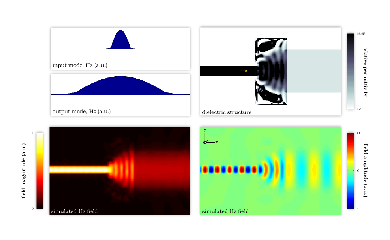
\includegraphics[width=0.8\textwidth]{1} 
    \caption{Coupler from a narrow, high-index ($\epsilon=12.25$) waveguide to
            a wide, low-index ($\epsilon=2.25$) waveguide. 
        The $H_z^\text{perfect}$ boundary values used as 
            the design objective are shown in the upper-left plots, 
            the generated structure is shown in the upper-right plot, and
            the simulated $H_z$ fields of the device are shown 
            in the bottom two plots.
        The computed efficiency of the coupler is high, $99.8\%$, and
            the device is also extremely compact, 
            convering only $36 \times 76$ grid points,
            where the vacuum wavelength is 42 grid points
            (footprint of $1.55$ square vacuum wavelengths).
        Computation time was 15 minutes on a personal computer.}
    \label{fig:fiber}
\end{figure}
\begin{figure}[htb]
    \centering
    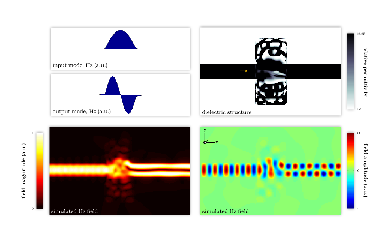
\includegraphics[width=0.8\textwidth]{2} 
    \caption{Coupler that converts the fundamental waveguide mode to the
            second-order waveguide mode
            (a movie of the design progress is included as a
            supplementary material).
        This problem is quite difficult since the two modes are of 
            opposite symmetry.
        For example, adiabatic approaches cannot be applied to this case.
        However, our method produces a device 
            (which has the same dimensions and vacuum wavelength as 
            Fig.~\ref{fig:fiber})  
            with a coupling efficiency of $98.0\%$. 
        Computation time was 15 minutes on a personal computer.
        }
    \label{fig:mode}
\end{figure}
\begin{figure}[htb]
    \centering
    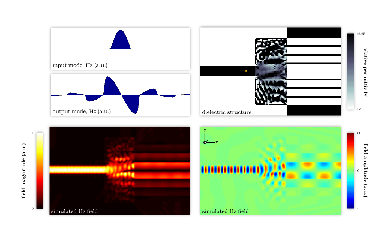
\includegraphics[width=0.8\textwidth]{3}
    \caption{Coupler between a dielectric slab waveguide to 
            an air-core waveguide.
        Here, not only are the modes of opposite symmetry,
            but the output waveguide operates on a fundamentally different
            principle (distributed reflection) than the input waveguide 
            (index guided).
        The device still achieves an efficiency of $98.9\%$, demonstrating the
            versatility of our method.
        The vacuum wavelength is 25 grid points, 
            while the device footprint is still $36 \times 76$ grid points
            (footprint of 4.38 square vacuum wavelengths).
        Computation time was 15 minutes on a personal computer.
        }
        \label{fig:aircore}
\end{figure}
\begin{figure}[htb]
    \centering
    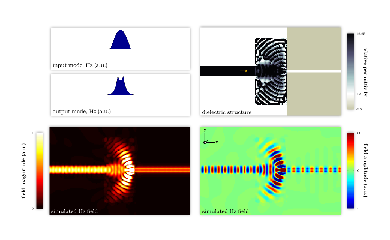
\includegraphics[width=0.8\textwidth]{4}
    \caption{Coupler between a dielectric slab waveguide to 
            a plasmonic metal-insulator-metal waveguide.
        The efficiency of the device is $97.5\%$ and 
            has the same wavelength and footprint as the device in
            Fig.~\ref{fig:aircore}.
        Computation time was 15 minutes on a personal computer.
        }
        \label{fig:mim}
\end{figure}
\clearpage
\begin{figure}[htb]
    \centering
    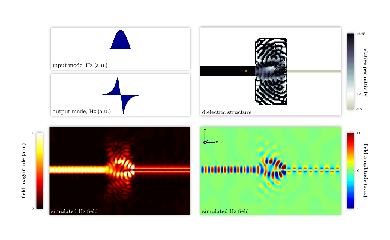
\includegraphics[width=0.8\textwidth]{5}
    \caption{Coupler between a dielectric slab waveguide to 
            a plasmonic wire waveguide.
        The efficiency of the device is $99.1\%$ and 
            has the same wavelength and footprint as the device in
            Fig.~\ref{fig:aircore}.
        Computation time was 15 minutes on a personal computer.
        }
        \label{fig:wire}
\end{figure}

\section{Conclusion}
We develop a fundamentally new approach to designing physical structures,
    which we term ``objective-first'', 
    in that we choose to satisfy the design objective 
    even above satisfying the physical equation which governs its operation.
We then apply this approach to the design of 
    various nanophotonic waveguide couplers,
    and show that our method produces
    high-efficiency designs ($\sim 98\%$ efficiency) 
    in small footprints (1.5-4 square vacuum wavelengths)
    without needing a good starting point.
Furthermore, we suggest that such a methodology may be applicable
    to the design of any single-mode, linear nanophotonic device.\\

This work has been supported by the 
    AFOSR MURI for Complex and Robust On-chip Nanophotonics 
    (Dr. Gernot Pomrenke), grant number FA9550-09-1-0704.
The Matlab code used is available online\cite{code}.
\clearpage
\begin{appendix}
\section{Additional mode coupler designs}
In this section, we present additional mode coupler designs.
A wide, high-index waveguide is used at both the input and output ports,
    and all permutations of couplers are fabricated among
    the first four propagating modes.
\begin{figure}[h!]
    \centering
    \includegraphics[width=0.8\textwidth]{6}
    \caption{
        Coupler from the first-order to the second-order mode 
            of a wide dielectric waveguide.
        Efficiency: $99.3\%$,
        footprint: $1.55$ square vacuum wavelengths.
        }
        % \label{fig:wire}
\end{figure}
\begin{figure}[h!]
    \centering
    \includegraphics[width=0.8\textwidth]{7}
    \caption{
        Coupler from the first-order to the third-order mode 
            of a wide dielectric waveguide.
        Efficiency: $98.3\%$,
        footprint: $1.55$ square vacuum wavelengths.
        }
        % \label{fig:wire}
\end{figure}
\begin{figure}[h!]
    \centering
    \includegraphics[width=0.8\textwidth]{8}
    \caption{
        Coupler from the first-order to the fourth-order mode 
            of a wide dielectric waveguide.
        Efficiency: $90.6\%$,
        footprint: $1.55$ square vacuum wavelengths.
        }
        % \label{fig:wire}
\end{figure}
\begin{figure}[h!]
    \centering
    \includegraphics[width=0.8\textwidth]{9}
    \caption{
        Coupler from the second-order to the third-order mode 
            of a wide dielectric waveguide.
        Efficiency: $96.8\%$,
        footprint: $1.55$ square vacuum wavelengths.
        }
        % \label{fig:wire}
\end{figure}
\begin{figure}[h!]
    \centering
    \includegraphics[width=0.8\textwidth]{10}
    \caption{
        Coupler from the second-order to the fourth-order mode 
            of a wide dielectric waveguide.
        Efficiency: $86.3\%$,
        footprint: $1.55$ square vacuum wavelengths.
        }
        % \label{fig:wire}
\end{figure}
\begin{figure}[h!]
    \centering
    \includegraphics[width=0.8\textwidth]{11}
    \caption{
        Coupler from the third-order to the fourth-order mode 
            of a wide dielectric waveguide.
        Efficiency: $80.1\%$,
        footprint: $1.55$ square vacuum wavelengths.
        }
        % \label{fig:wire}
\end{figure}
\clearpage
\section{Additional designs with wide, low-index input waveguide}
We now reproduce Figs~\ref{fig:mode}-\ref{fig:wire}
    but instead use a wide, low-index waveguide as the input.
Once again, this is to demonstrate the generality of our method;
    namely, that it can be applied to the design of nearly any
    single-mode, linear nanophotonic device.
\begin{figure}[h!]
    \centering
    \includegraphics[width=0.8\textwidth]{12}
    \caption{
        Coupler from a wide, low-index waveguide to the
            second-order mode of a narrow, high-index waveguide.
        Efficiency: $96.9\%$,
        footprint: $1.55$ square vacuum wavelengths.
        }
        % \label{fig:wire}
\end{figure}
\begin{figure}[h!]
    \centering
    \includegraphics[width=0.8\textwidth]{13}
    \caption{
        Coupler from a wide, low-index waveguide to an 
            ``air-core'' waveguide mode.
        Efficiency: $99.0\%$,
        footprint: $4.38$ square vacuum wavelengths.
        }
        % \label{fig:wire}
\end{figure}
\begin{figure}[h!]
    \centering
    \includegraphics[width=0.8\textwidth]{14}
    \caption{
        Coupler from a wide, low-index waveguide to a
            metal-insulator-metal plasmonic waveguide mode.
        Efficiency: $96.7\%$,
        footprint: $4.38$ square vacuum wavelengths.
        }
        % \label{fig:wire}
\end{figure}
\begin{figure}[h!]
    \centering
    \includegraphics[width=0.8\textwidth]{15}
    \caption{
        Coupler from a wide, low-index waveguide to a
            plasmonic wire waveguide mode.
        Efficiency: $99.7\%$,
        footprint: $4.38$ square vacuum wavelengths.
        }
        % \label{fig:wire}
\end{figure}
\clearpage

\section{Additional designs with multiple output plasmonic waveguides}
We also present ``selector'' designs where photons are coupled to 
    only one of five possible plasmonic output waveguides.
We demonstrate these selector designs for both metal-insulator-metal and
    metal-wire plasmonic waveguides.
\begin{figure}[h!]
    \centering
    \includegraphics[width=0.8\textwidth]{16}
    \caption{
        Coupler from a dielectric waveguide to the 
            lowest branch of a set of five plasmonic wire waveguides.
        Efficiency: $94.0\%$,
        footprint: $4.38$ square vacuum wavelengths.
        }
        % \label{fig:wire}
\end{figure}
\begin{figure}[h!]
    \centering
    \includegraphics[width=0.8\textwidth]{17}
    \caption{
        Coupler from a dielectric waveguide to the 
            second branch of a set of five plasmonic wire waveguides.
        Efficiency: $97.3\%$,
        footprint: $4.38$ square vacuum wavelengths.
        }
        % \label{fig:wire}
\end{figure}
\begin{figure}[h!]
    \centering
    \includegraphics[width=0.8\textwidth]{18}
    \caption{
        Coupler from a dielectric waveguide to the 
            middle branch of a set of five plasmonic wire waveguides.
        Efficiency: $98.5\%$,
        footprint: $4.38$ square vacuum wavelengths.
        }
        % \label{fig:wire}
\end{figure}
\begin{figure}[h!]
    \centering
    \includegraphics[width=0.8\textwidth]{19}
    \caption{
        Coupler from a dielectric waveguide to the 
            middle branch of a set of five plasmonic 
            metal-insulator-metal waveguides.
        Efficiency: $97.7\%$,
        footprint: $4.38$ square vacuum wavelengths.
        }
        % \label{fig:wire}
\end{figure}
\begin{figure}[h!]
    \centering
    \includegraphics[width=0.8\textwidth]{20}
    \caption{
        Coupler from a dielectric waveguide to the 
            fourth branch of a set of five plasmonic 
            metal-insulator-metal waveguides.
        Efficiency: $95.6\%$,
        footprint: $4.38$ square vacuum wavelengths.
        }
        % \label{fig:wire}
\end{figure}
\begin{figure}[h!]
    \centering
    \includegraphics[width=0.8\textwidth]{21}
    \caption{
        Coupler from a dielectric waveguide to the 
            uppermost branch of a set of five plasmonic 
            metal-insulator-metal waveguides.
        Efficiency: $87.5\%$,
        footprint: $4.38$ square vacuum wavelengths.
        }
        % \label{fig:wire}
\end{figure}
\clearpage
\end{appendix}
\end{document}

